\mysection{Функция toupper()}
\myindex{\CStandardLibrary!toupper()}

Еще одна очень востребованная функция конвертирует символ из строчного в заглавный, если нужно:

\lstinputlisting[style=customc]{\CURPATH/toupper.c}

Выражение \TT{'a'+'A'} оставлено в исходном коде для удобства чтения, 
конечно, оно соптимизируется

\footnote{Впрочем, если быть дотошным, вполне могут до сих пор существовать компиляторы,
которые не оптимизируют подобное и оставляют в коде.}.

\ac{ASCII}-код символа \q{a} это 97 (или 0x61), и 65 (или 0x41) для символа \q{A}.

Разница (или расстояние) между ними в \ac{ASCII}-таблице это 32 (или 0x20).

Для лучшего понимания, читатель может посмотреть на стандартную 7-битную таблицу \ac{ASCII}:

\begin{figure}[H]
\centering
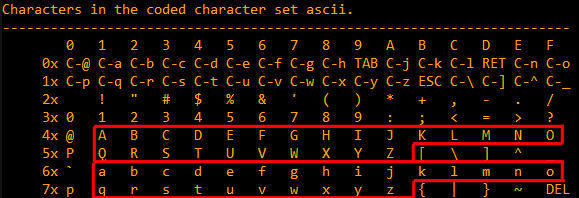
\includegraphics[width=0.8\textwidth]{ascii.png}
\caption{7-битная таблица \ac{ASCII} в Emacs}
\end{figure}

\subsection{x64}

\subsubsection{Две операции сравнения}

\NonOptimizing MSVC прямолинеен: код проверят, находится ли входной символ в интервале [97..122]
(или в интервале [`a'..`z'] ) и вычитает 32 в таком случае.

Имеется также небольшой артефакт компилятора:

\lstinputlisting[caption=\NonOptimizing MSVC 2013 (x64),numbers=left,style=customasmx86]{\CURPATH/MSVC_2013_x64_RU.asm}

Важно отметить что (на строке 3) входной байт загружается в 64-битный слот локального стека.

Все остальные биты ([8..63]) не трогаются, т.е. содержат случайный шум (вы можете увидеть его в отладчике).
% TODO add debugger example

Все инструкции работают только с байтами, так что всё нормально.

Последняя инструкция \TT{MOVZX} на строке 15 берет байт из локального стека и расширяет его 
до 32-битного \Tint, дополняя нулями.

\NonOptimizing GCC делает почти то же самое:

\lstinputlisting[caption=\NonOptimizing GCC 4.9 (x64),style=customasmx86]{\CURPATH/GCC_49_x64_O0.s}

\subsubsection{Одна операция сравнения}
\label{toupper_one_comparison}

\Optimizing MSVC работает лучше, он генерирует только одну операцию сравнения:

\lstinputlisting[caption=\Optimizing MSVC 2013 (x64),style=customasmx86]{\CURPATH/MSVC_2013_Ox_x64.asm}

Уже было описано, как можно заменить две операции сравнения на одну: \myref{one_comparison_instead_of_two}.

Мы бы переписал это на \CCpp так:

\begin{lstlisting}[style=customc]
int tmp=c-97;

if (tmp>25)
        return c;
else
        return c-32;
\end{lstlisting}

Переменная \emph{tmp} должна быть знаковая.

При помощи этого, имеем две операции вычитания в случае конверсии плюс одну операцию сравнения.

В то время как оригинальный алгоритм использует две операции сравнения плюс одну операцию вычитания.

\Optimizing GCC 
даже лучше, он избавился от переходов (а это хорошо: \myref{branch_predictors}) используя инструкцию CMOVcc:

\lstinputlisting[caption=\Optimizing GCC 4.9 (x64),numbers=left,style=customasmx86,label=toupper_GCC_O3]{\CURPATH/GCC_49_x64_O3.s}

На строке 3 код готовит уже сконвертированное значение заранее, как если бы конверсия всегда происходила.

На строке 5 это значение в EAX заменяется нетронутым входным значением, если конверсия не нужна.
И тогда это значение (конечно, неверное), просто выбрасывается.

Вычитание с упреждением это цена, которую компилятор платит за отсутствие условных переходов.

\subsection{ARM}

\Optimizing Keil для режима ARM также генерирует только одну операцию сравнения:

\lstinputlisting[caption=\OptimizingKeilVI (\ARMMode),style=customasmARM]{\CURPATH/Keil_ARM_O3.s}

\myindex{ARM!\Instructions!SUBcc}
\myindex{ARM!\Instructions!ANDcc}

\INS{SUBLS} и \INS{ANDLS} исполняются только если значение \Reg{1} меньше чем 0x19 (или равно).
Они и делают конверсию.

\Optimizing Keil для режима Thumb также генерирует только одну операцию сравнения:

\lstinputlisting[caption=\OptimizingKeilVI (\ThumbMode),style=customasmARM]{\CURPATH/Keil_thumb_O3.s}

\myindex{ARM!\Instructions!LSLS}
\myindex{ARM!\Instructions!LSLR}

Последние две инструкции \INS{LSLS} и \INS{LSRS} работают как \INS{AND reg, 0xFF}:
это аналог \CCpp-выражения $(i<<24)>>24$.

Очевидно, Keil для режима Thumb решил, что две 2-байтных инструкции это короче чем код, загружающий
константу 0xFF плюс инструкция AND.

\subsubsection{GCC для ARM64}

\lstinputlisting[caption=\NonOptimizing GCC 4.9 (ARM64),style=customasmARM]{\CURPATH/GCC_49_ARM64_O0.s}

\lstinputlisting[caption=\Optimizing GCC 4.9 (ARM64),style=customasmARM]{\CURPATH/GCC_49_ARM64_O3.s}

\subsection{Используя битовые операции}
\label{toupper_bit}

Учитывая тот факт, что 5-й бит (считая с 0-го) всегда присутствует после проверки, вычитание его это просто
сброс этого единственного бита, но точно такого же эффекта можно достичть при помощи обычного применения операции
``И''.

И даже проще, с исключающим ИЛИ:

\lstinputlisting[style=customc]{\CURPATH/toupper2.c}

Код близок к тому, что сгенерировал оптимизирующий GCC для предыдущего примера (\myref{toupper_GCC_O3}):

\lstinputlisting[caption=\Optimizing GCC 5.4 (x86),style=customasmx86]{\CURPATH/toupper2_GCC540_x86_O3.s}

\dots но используется \INS{XOR} вместо \INS{SUB}.

Переворачивание 5-го бита это просто перемещение \textit{курсора} в таблице \ac{ASCII} вверх/вниз на 2 ряда.

Некоторые люди говорят, что буквы нижнего/верхнего регистра были расставлены в \ac{ASCII}-таблице таким манером намеренно,
потому что:

\begin{framed}
\begin{quotation}
Very old keyboards used to do Shift just by toggling the 32 or 16 bit, depending on the key; this is why the relationship between small and capital letters in ASCII is so regular, and the relationship between numbers and symbols, and some pairs of symbols, is sort of regular if you squint at it.
\end{quotation}
\end{framed}

( Eric S. Raymond, \url{http://www.catb.org/esr/faqs/things-every-hacker-once-knew/} )

Следовательно, мы можем написать такой фрагмент кода, который просто меняет регистр букв:

\lstinputlisting[style=customc]{\CURPATH/flip_RU.c}

\subsection{Итог}

Все эти оптимизации компиляторов очень популярны в наше время и практикующий
reverse engineer обычно часто видит такие варианты кода.
